\chapter{Trigonometrie}
\section{Kurze Wiederholung}
\begin{Bws}
Im Kreis mit Radius 1 gelte:\\
\cos(\alpha)= x_{_M}\\
\sin(\alpha)= y_{_M}
\end{Bws}
%Punkt M einzeichnen!
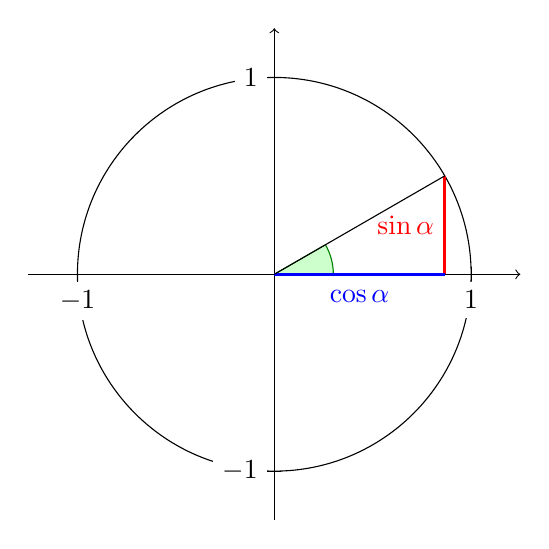
\begin{tikzpicture}[scale=2.5]
\filldraw[fill=green!20,draw=green!50!black] (0,0) -- (3mm,0mm) arc (0:30:3mm) -- cycle;
\draw[->] (-1.25,0) -- (1.25,0) coordinate (x axis);
\draw[->] (0,-1.25) -- (0,1.25) coordinate (y axis);
\draw (0,0) circle (1cm);
\draw[very thick,red] (30:1cm) -- node[left,fill=white] {$\sin \alpha$} (30:1cm |- x axis);
\draw[very thick,blue] (30:1cm |- x axis) -- node[below=2pt,fill=white] {$\cos\alpha$} (0,0);
\draw (0,0) -- (30:1cm);
\foreach \x/\xtext in {-1, 1}
\draw (\x cm,1pt) -- (\x cm,-1pt) node[anchor=north,fill=white] {$\xtext$};
\foreach \y/\ytext in {-1, 1}
\draw (1pt,\y cm) -- (-1pt,\y cm) node[anchor=east,fill=white] {$\ytext$};
\end{tikzpicture}
\\
Es ergeben sich folgende (wissenswerte) Werte:




\section{Polarkoordinaten}
adf
\section{Addtions- und Versopplungssätze}
\begin{Bws}
$cos(a - b) = cos(a)cos(b) + sin(a) sin(b)$\\
$sin(a - b) = sin(a)cos(b) - cos(a)sin(b)$\\
$cos(a + b) = cos(a)cos(b) - sin(a)sin(b)$\\
$sin(a + b) = sin(a)cos(b) + cos(a)sin(b)$
\end{Bws}

\section{Allgemeine Sinus- und Kosinussätze}
Dreieck malen! \\
Diese Sätze gelten in einem beliebigen Dreieck:
\begin{Bws}
$\dfrac {a} {sin(\alpha)}=\dfrac {b} {sin(\beta)}=\dfrac {c} {sin(\gamma)}$\\\\
$c²=a²+b²-2abcos(\gamma)$
\end{Bws}
Man bemerkt, dass sich die bekannten Relationen ergeben, wenn man für einen der Winkel den Wert $\dfrac{\pi}{2}$ nimmt.
